
\section{CONCLUSION AND FUTURE PROSPECTS}
In this paper, we have proposed a method of path-finding for platonic solids - regular convex polyhedra - under rolling constraint without sliding. Using tree exploration algorithm can find the path for cube, tetrahedron, octahedron and icosahedron solids. In the first case of dodecahedron with a gap between two pentagons in the initial environment, the algorithm is be applied to find shortest paths while the other case with overlaps is not guaranteed to find a path.\\


\noindent The results of this study concern path planning in discrete environment through rolling for only platonic solids with free-obstacles.
In future work some more case studies can be included such as rolling platonic solids with obstacles in the environment, optimal algorithm with reducing the cost of memory while executing the algorithm.\\

%\textcolor{blue}{
%\uline{Questions}: Q4. Why should the community care?\\
%\noindent\uline{Should do}: 
%- Overview of Q1, Q2, and Q3; plus\\
%- What does the community still not know?\\
%}
%
%\noindent\uline{Examples}:
%- We have introduced a method of ....\\
%- Most of our effort has focused on .... The results of our method often contain .... We believe that there is significant room for improvement by applying ABC methods to the XYZ problem.\\
%- What do we not do?\\
%
%In this study, we established a method for ... Although we focused on discrete path planning of platonic solid - regular convex polyhedra in known environment, as illustrated using ABC model and EFG example, the developed method/algorithm can be easily implemented to the complex convex polyhedra such as elipsoil ???. The contributions of this study can be summarized as follows:\\
%
%\begin{figure}[h]
%\centering
%	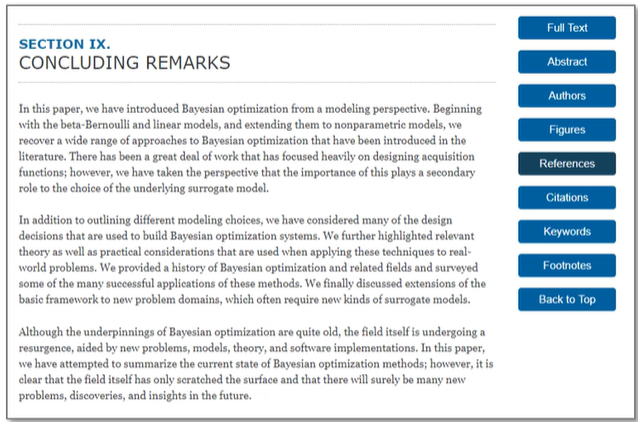
\includegraphics[width=1\textwidth]{image/IEEEDisCon}
%	\caption{First four paths of the cube rolling}
%	\label{fig:Tetra2Case1}
%\end{figure}
